\documentclass{beamer}
\usetheme{Boadilla}
\usepackage[norsk]{babel}
\usepackage[utf8]{inputenc}
\usepackage{url}
\usepackage{hyperref}
\usepackage{subfig}

%\usepackage[square,sort,comma,numbers]{natbib}
\usepackage{bibentry}
\nobibliography*
\bibliographystyle{ieeetr}

\title{PheroMusic}
\author{Håkon Knutzen}
\institute[IFI,UiO] 
{
	\centering
	
\includegraphics[scale=.4]{pics/UiO_Segl_pms485.eps}	
	
	
\includegraphics[scale=.2]{pics/logo_epics.pdf}
}
\date{}
\begin{document}

\begin{frame}[plain]
	\titlepage
\end{frame}

\begin{frame}
	\frametitle{PheroMusic-appen}
	\begin{figure}
	\centering
	\subfloat[Hovedvindu \label{fig:ss:app:a}]{\fbox{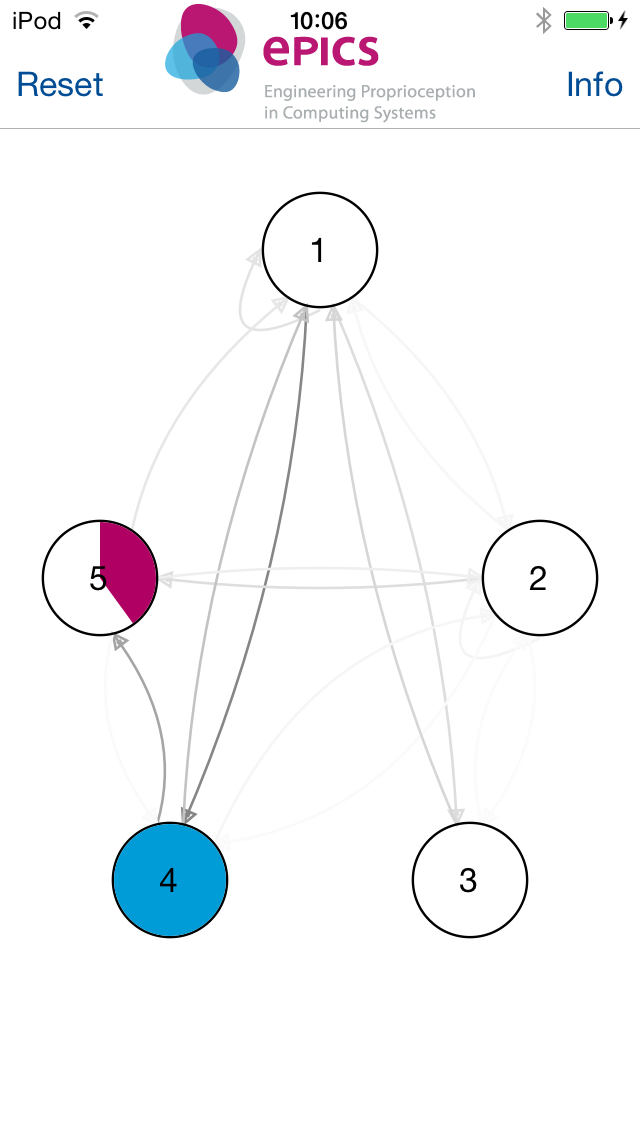
\includegraphics[width = .25\textwidth]{pics/view1.png}}}\hspace{5pt}
	\subfloat[Infovindu \label{fig:ss:app:b}]{\fbox{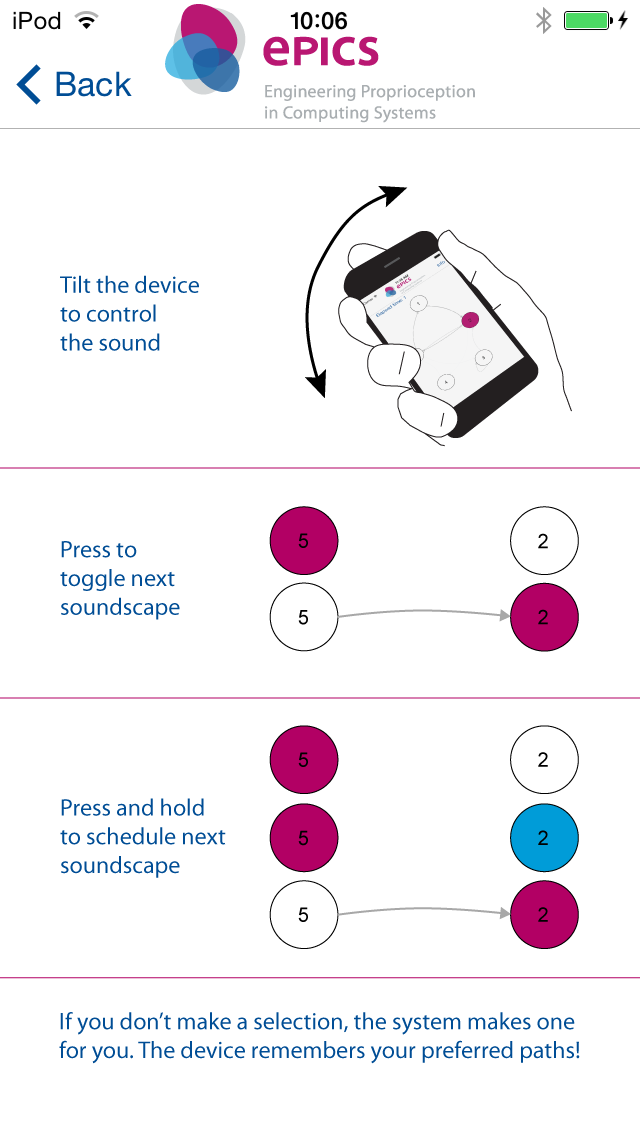
\includegraphics[width = .25\textwidth]{pics/view2.png}}}
	\caption{\label{fig:ss:app} Skjermbilde av appen.}
	\end{figure}
\end{frame}

\begin{frame}
	\frametitle{Funksjonalitet}
	\begin{itemize}[<+->]
		\item ``Aktiv musikk''
		\item Fem noder kan velges eller settes i kø
		\item Styr parametre i musikken ved å tilte enheten
		\item Enheten skal kunne foreta et valg basert på tidligere valg
	\end{itemize}
\end{frame}

\begin{frame}
	\frametitle{Algoritmen}
	\begin{itemize}[<+->]
		\item Biologisk inspirert algoritme
		\item En ``maur'' legger fra seg et feromonspor som fordamper
		\item Tabell med verdier som representerer koblinger. Vises i grafisk ved å tegne stiene mellom nodene
	\end{itemize}
\end{frame}

\begin{frame}[allowframebreaks]
	\frametitle{Overgangssannsynlighet}
	\begin{table}
		\caption{En feromontabell.\label{tbl:pheromone}}
		\centering
		\begin{tabular}{c | c c c c c }
			& 1 & 2 & 3 & 4 & 5 \\
			\hline
			1 & 3 & 2 & 7 & 9 & 3 \\
			2 & 1 & 2 & 1 & 3 & 4 \\
			3 & 2 & 2 & 1 & 3 & 6 \\
			4 & 1 & 1 & 9 & 2 & 3 \\
			5 & 7 & 1 & 2 & 2 & 4 \\
		\end{tabular}
	\end{table}
	\begin{figure}
		\fbox{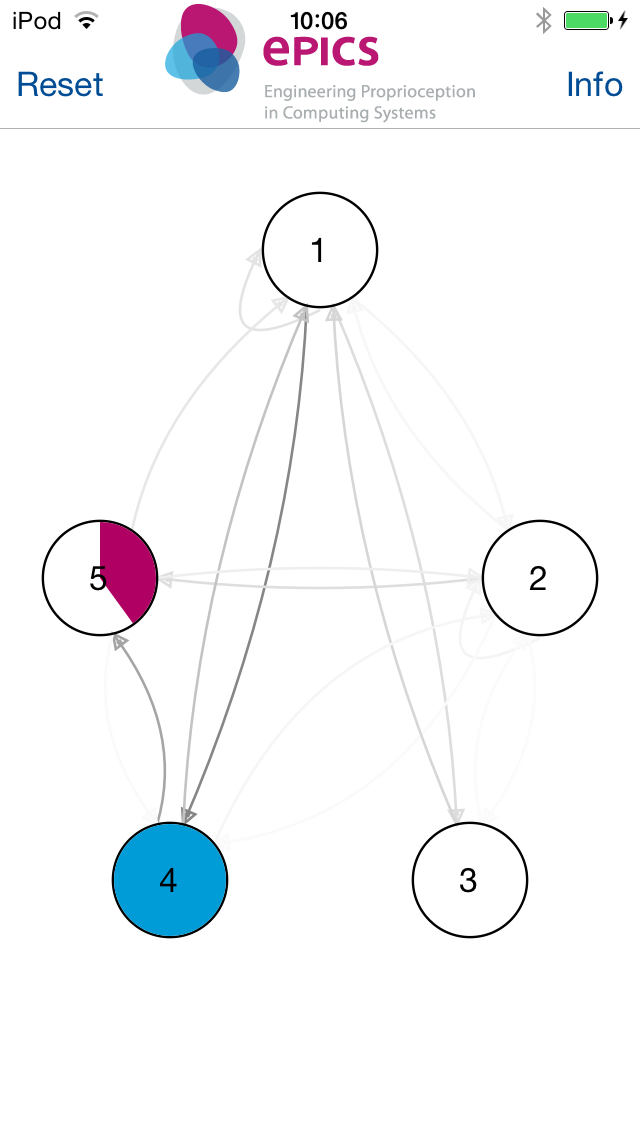
\includegraphics[scale=.15]{pics/view1.png}}
		\caption{Sterke koblinger er synligst}
	\end{figure}
\end{frame}

\begin{frame}
	\frametitle{Implementasjon}
	\begin{itemize}[<+->]
		\item Basert på et konsept som var implementert med Max MSP (lyd), Processing (grafikk) og Mobmuplat (kontroll)\footnote{\bibentry{Nymoen:2014b}}
		\item Implementert som selvstendig app for iOS:
		\begin{itemize}
			\item Algoritme og UI: Objective-C/Cocoa touch
			\item Lyd: Puredata/libpd
		\end{itemize}
	\end{itemize}
\end{frame}

\begin{frame}
	\frametitle{Lydlandsskaper (soundscapes)}
	\begin{itemize}[<+->]
		\item En slags mini-DAW:
			\begin{itemize}
				\item Sanntidssyntese
				\item Avspilling av lyder
				\item Filtrering
				\item Romklangbus
				\item Masterbus med komprimering
			\end{itemize}
		\item En-til-mange mapping: Pitch$\rightarrow$flere synthparametre
	\end{itemize}
\end{frame}




\begin{frame}
	\frametitle{Last ned og prøv}
	\centering
	
\includegraphics[scale=.3]{pics/document.pdf}
\end{frame}

\begin{frame}[allowframebreaks]

\bibliography{refs}

\end{frame}




\end{document}